\chapter{Análise Pós-Laboratorial e Resultados}

A fase de pós-processamento de dados visa reconciliar o modelo matemático ideal desenvolvido na análise teórica com a realidade fenomênica observada na bancada. Em consonância com as diretrizes da prática, o procedimento analítico a seguir contempla a reavaliação das funções de transferência a partir dos componentes reais, o cômputo do ganho experimental e a sobreposição gráfica no diagrama de Bode.

\section{Recálculo das Funções de Transferência}

A tolerância intrínseca aos processos de fabricação dos componentes passivos introduz desvios na alocação dos polos do sistema. Para eliminar o erro paramétrico na sobreposição gráfica, a função de transferência geral $H(s)$ deduzida anteriormente foi reavaliada no ambiente de computação simbólica Maxima \cite{maxima}, inserindo-se as grandezas elétricas medidas a frio com o multímetro Keysight U1253B.

\subsection{Primeiro Circuito (Superamortecido)}

Utilizando os valores da Tabela \ref{tab:componentes_c1} ($R_1 = 47,13\text{ k}\Omega$, $R_2 = 469,4\text{ k}\Omega$, $R_3 = 478,0\text{ k}\Omega$, $C_1 = 109,9\text{ nF}$ e $C_2 = 11,42\text{ nF}$), o ganho DC estático nominal, que era de $-10\text{ V/V}$, foi ligeiramente alterado no circuito real para:
\begin{equation}
	A_{v(real)} = -\frac{R_2}{R_1} = -\frac{469,4\text{ k}\Omega}{47,13\text{ k}\Omega} \approx -9,96 \text{ V/V}
\end{equation}
Estes dados foram injetados no \textit{script} do Maxima para gerar a curva logarítmica contínua recalculada do filtro passa-baixa.

\subsection{Segundo Circuito (Subamortecido)}

Aplicando a mesma metodologia para os valores da Tabela \ref{tab:componentes_c2} ($R_1 = 469,4\text{ k}\Omega$, $R_2 = 478,0\text{ k}\Omega$, $R_3 = 47,13\text{ k}\Omega$), o ganho estático deste estágio manteve-se próximo do unitário:
\begin{equation}
	A_{v(real)} = -\frac{R_2}{R_1} = -\frac{478,0\text{ k}\Omega}{469,4\text{ k}\Omega} \approx -1,01 \text{ V/V}
\end{equation}
O recálculo paramétrico refina a localização precisa da frequência de pico de ressonância teórica, aproximando o traçado matemático ao evento físico medido em $17,5\text{ Hz}$.

\section{Estimativa Experimental da Magnitude}

Para cada ponto do espectro de frequência amostrado no laboratório, a magnitude empírica da função de transferência (ganho em módulo) foi determinada pela razão direta entre a amplitude da tensão de saída e a amplitude da tensão de entrada ($|H| = V_{out} / V_{in}$). 

As Tabelas \ref{tab:magnitude_c1} e \ref{tab:magnitude_c2} consolidam essas estimativas experimentais para ambos os circuitos.

\begin{table}[H]
	\centering
	\caption{Cálculo da magnitude experimental $|H(j\omega)|$ - Circuito 1.}
	\label{tab:magnitude_c1}
	\renewcommand{\arraystretch}{1.2}
	\begin{tabular}{cccc}
		\hline
		\textbf{Frequência Aplicada} & \textbf{Tensão $V_{in}$ (mV)} & \textbf{Tensão $V_{out}$ (mV)} & \textbf{Magnitude Estimada ($|H|$)} \\ \hline
		$0,6\text{ Hz}$ & $78$ & $750$ & $9,62$ \\
		$1,7\text{ Hz}$ & $132$ & $1050$ & $7,95$ \\
		$2,5\text{ Hz}$ & $143$ & $960$ & $6,71$ \\
		$4,3\text{ Hz}$ ($f_1$) & $152$ & $730$ & $4,80$ \\
		$5,2\text{ Hz}$ & $153$ & $640$ & $4,18$ \\
		$6,0\text{ Hz}$ & $153$ & $570$ & $3,73$ \\
		$7,7\text{ Hz}$ & $154$ & $460$ & $2,99$ \\
		$10,8\text{ Hz}$ & $154$ & $340$ & $2,21$ \\
		$17,2\text{ Hz}$ & $155$ & $210$ & $1,35$ \\
		$25,8\text{ Hz}$ & $155$ & $140$ & $0,90$ \\
		$43,0\text{ Hz}$ & $155$ & $60$ & $0,39$ \\ \hline
	\end{tabular}
\end{table}

\begin{table}[H]
	\centering
	\caption{Cálculo da magnitude experimental $|H(j\omega)|$ - Circuito 2.}
	\label{tab:magnitude_c2}
	\renewcommand{\arraystretch}{1.2}
	\begin{tabular}{cccc}
		\hline
		\textbf{Frequência Aplicada} & \textbf{Tensão $V_{in}$ (V)} & \textbf{Tensão $V_{out}$ (V)} & \textbf{Magnitude Estimada ($|H|$)} \\ \hline
		$2,6\text{ Hz}$ & $4,7$ & $4,7$ & $1,00$ \\
		$7,0\text{ Hz}$ & $5,0$ & $5,0$ & $1,00$ \\
		$10,5\text{ Hz}$ & $5,0$ & $5,1$ & $1,02$ \\
		$17,5\text{ Hz}$ ($f_{max}$) & $5,0$ & $5,0$ & $1,00$ \\
		$21,0\text{ Hz}$ & $5,0$ & $4,7$ & $0,94$ \\
		$24,5\text{ Hz}$ & $5,0$ & $4,6$ & $0,92$ \\
		$31,0\text{ Hz}$ & $5,0$ & $3,9$ & $0,78$ \\
		$43,7\text{ Hz}$ & $5,0$ & $2,7$ & $0,54$ \\
		$70,0\text{ Hz}$ & $5,0$ & $1,3$ & $0,26$ \\
		$105,0\text{ Hz}$ & $5,0$ & $0,6$ & $0,12$ \\
		$175,0\text{ Hz}$ & $5,1$ & $0,22$ & $0,04$ \\ \hline
	\end{tabular}
\end{table}

\section{Sobreposição Gráfica e Diagrama de Bode}

A validação final do comportamento do circuito foi obtida por meio da plotagem, em escala \textit{log-log}, dos dados experimentais pontuais sobrepostos à curva analítica recalculada do módulo de $H(j\omega)$. O processo gráfico foi automatizado utilizando o \textit{script} base do Maxima fornecido na disciplina.

As Figuras \ref{fig:bode_c1} e \ref{fig:bode_c2} apresentam a correspondência entre a modelagem ajustada e as medições empíricas.

\begin{figure}[H]
	\centering
	% Substitua esta imagem pela exportação gráfica gerada no Maxima para o Circuito 1
	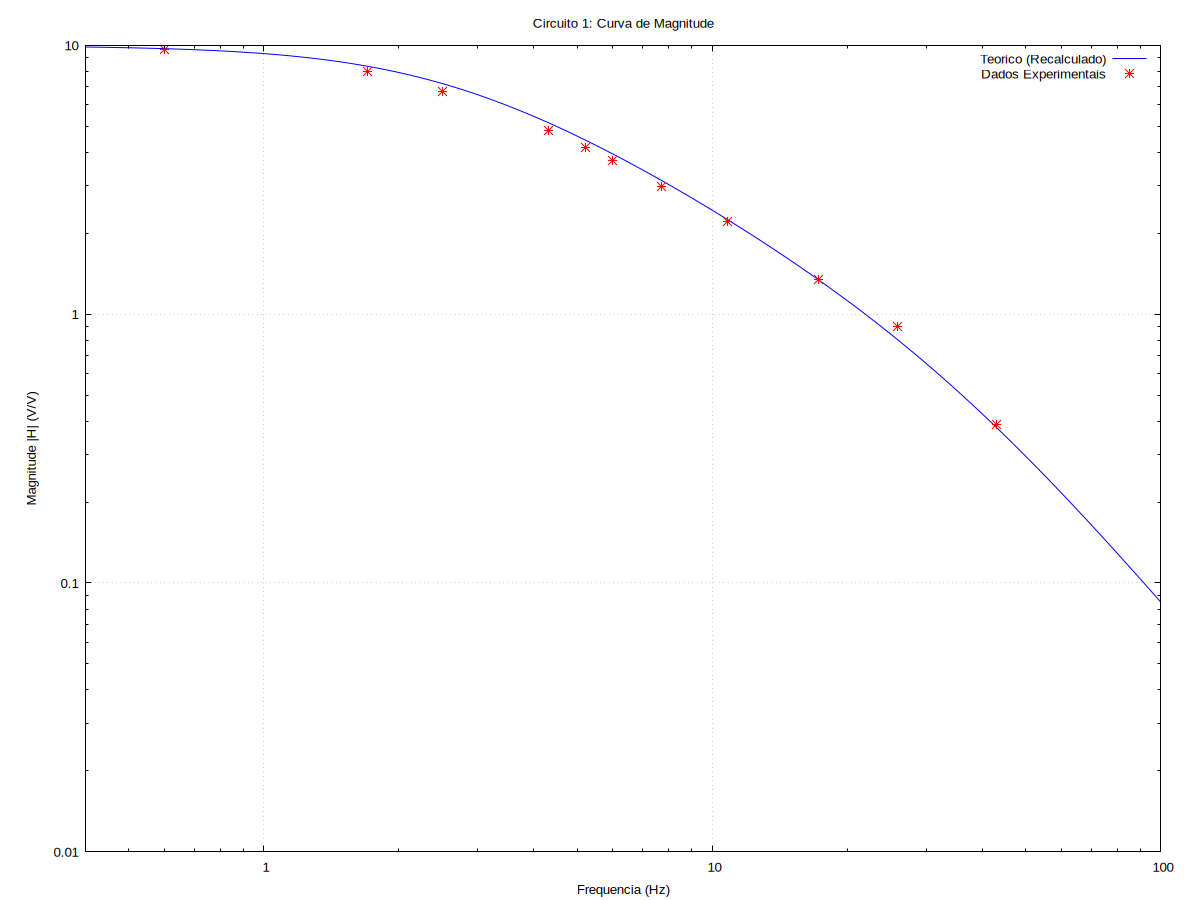
\includegraphics[width=0.8\textwidth]{FIGURAS/bode_plot_c1.png}
	%\fbox{\vspace{5cm} [ INSERIR GRÁFICO DE BODE LOG-LOG GERADO NO MAXIMA - CIRCUITO 1 ] \vspace{5cm}}
	\caption{Diagrama de Bode de magnitude: sobreposição da curva teórica recalculada com os pontos medidos experimentalmente (Circuito 1).}
	\label{fig:bode_c1}
\end{figure}

\begin{figure}[H]
	\centering
	% Substitua esta imagem pela exportação gráfica gerada no Maxima para o Circuito 2
	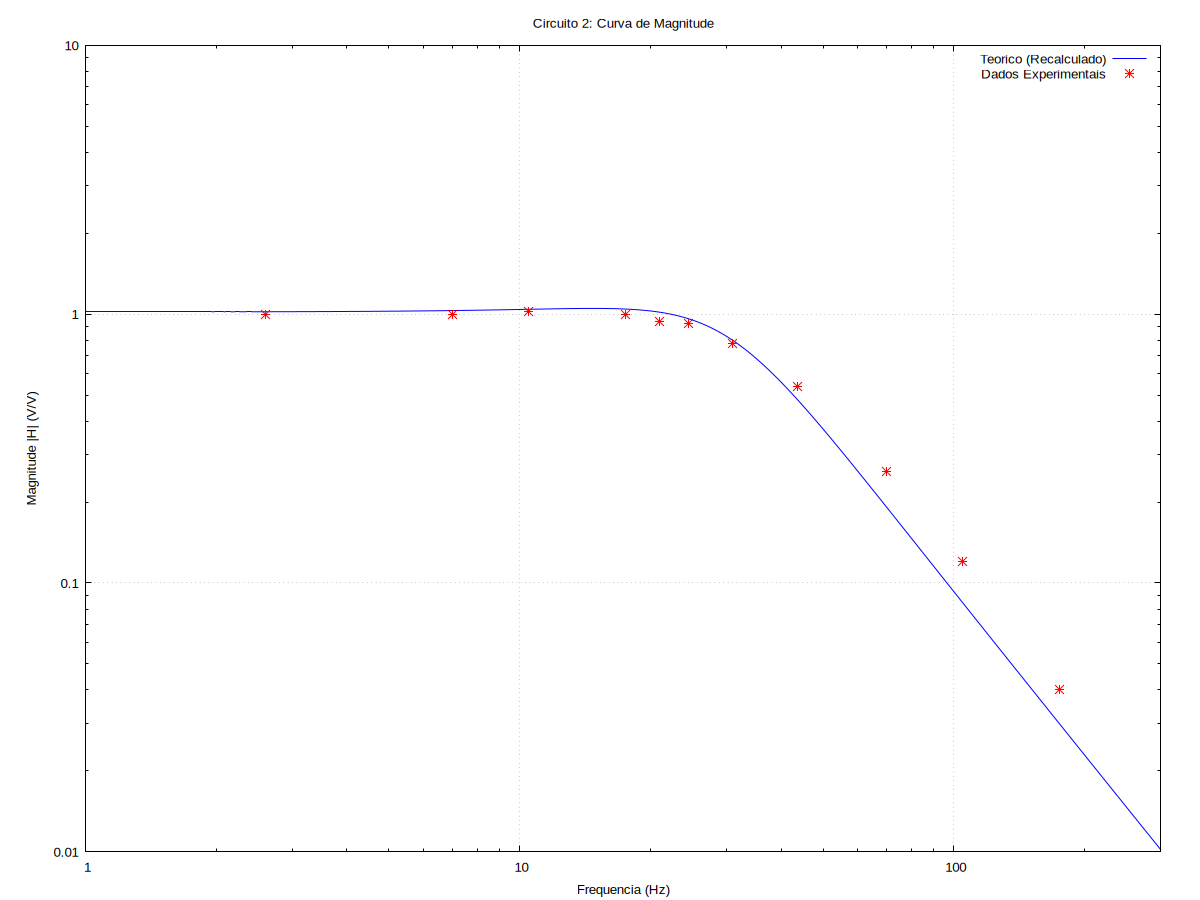
\includegraphics[width=0.8\textwidth]{FIGURAS/bode_plot_c2.png}
	%\fbox{\vspace{5cm} [ INSERIR GRÁFICO DE BODE LOG-LOG GERADO NO MAXIMA - CIRCUITO 2 ] \vspace{5cm}}
	\caption{Diagrama de Bode de magnitude: sobreposição da curva teórica recalculada destacando o pico de ressonância com os pontos medidos experimentalmente (Circuito 2).}
	\label{fig:bode_c2}
\end{figure}

\section{Análise de Divergências e Fontes de Erro}

A inspeção dos dados processados revela um alto grau de aderência estrutural entre a teoria ajustada e a prática, atestando a validade do modelo ideal para circuitos com frequências contidas na largura de banda do amplificador operacional. Contudo, os discretos desvios observados (como a variação do pico real para $17,5\text{ Hz}$) emanam das seguintes naturezas:

\begin{itemize}
	\item \textbf{Efeito de Carga e Instrumentação:} Pequenas perdas de sinal ($V_{in}$) nas frequências mais altas e mais baixas sugerem a flutuação da impedância de saída do gerador de sinais associada às resistências e capacitâncias parasitas da \textit{protoboard} de montagem.
	\item \textbf{Resolução de Leitura Visual:} A extração do valor de pico a pico no osciloscópio, especialmente quando acompanhada por ruídos de baixa frequência da rede ($\approx 60\text{ Hz}$), induz uma incerteza de quantização humana de alguns milivolts.
	\item \textbf{Não-Idealidades do OP-AMP:} Embora o modelo assuma $A \to \infty$ e Produto Ganho-Banda ilimitado, o circuito integrado real introduz pequenos pólos indesejados em frequências superiores, bem como correntes de polarização e de deslocamento (\textit{offset}) que afetam o patamar dinâmico estrito \cite{nilsson}.
\end{itemize}